\chapter{Exemplo}

\section{Tabela com o Pacote Booktabs}

Um exemplo de tabela com o pacote booktabs pode ser visto na Tabela \ref{tabela:exemplo}. A explica��o das tabelas sempre vem em cima e esse padr�o deve ser respeitado. A numera��o � autom�tica e a inser��o no �ndice tamb�m. Legal n�? \cite{Bennett:QuantumInformationSurvey}

Basta quebrar uma linha para criar um novo par�grafo. Neste par�grafo vou contar que tabelas no \LaTeX d�o um pouco de trabalho, mas nada que com paci�ncia n�o se resolva. Veja os links com dicas que coloquei nos coment�rios do arquivo \texttt{index.tex}.

\begin{table}[ht!]
\caption{Esta � uma tabela b�sica em \LaTeX com o pacote booktabs.} \label{tabela:exemplo}
\center{
\begin{tabular}{cccc}
\toprule
Parte 1 & Parte 2 & Parte 3 & Parte 4\\
\midrule
0,415 & 1,365 & 1,98 & 2,05\\
1,36  & 45,5  & 7,98 & 3,01\\
2,36  & 1,35  & 0,15 & 5,32\\
\bottomrule
\end{tabular}}
\end{table}



\section{Inser��o de Figuras}

Voc� pode inserir figuras JPG no \LaTeX! Veja o caso da Figura \ref{fig:exemplo}. Se voc� quiser outras configura��es e dicas, veja o seguinte endere�o: \url{http://en.wikibooks.org/wiki/LaTeX/Floats,_Figures_and_Captions}.

A explica��o da figura sempre vem embaixo da mesma. Isto aqui � um novo par�grafo apenas para ilustrar a id�ia geral de como escrever.

\begin{figure}[H]
\centering
\caption{Um exemplo de figura JPG inserida no \LaTeX.} \label{fig:exemplo}
\includegraphics[width=0.4\textwidth]{./img/exemplo.jpg}\\
\small{Elaborado pelo autor.}
\end{figure}

Pode inserir v�rias figuras lado a lado tamb�m. Um exemplo est� reproduzido a seguir.

\begin{figure}[H]
  \centering
  \caption{Canal cl�ssico cuja obten��o da capacidade erro-zero � n�o-trivial.}
  \subfloat[\ ]{\label{fig:exG5}\includegraphics[width=0.3\textwidth]{./img/001}}
  \hspace{0.5cm}
  \subfloat[\ ]{\label{fig:exG52}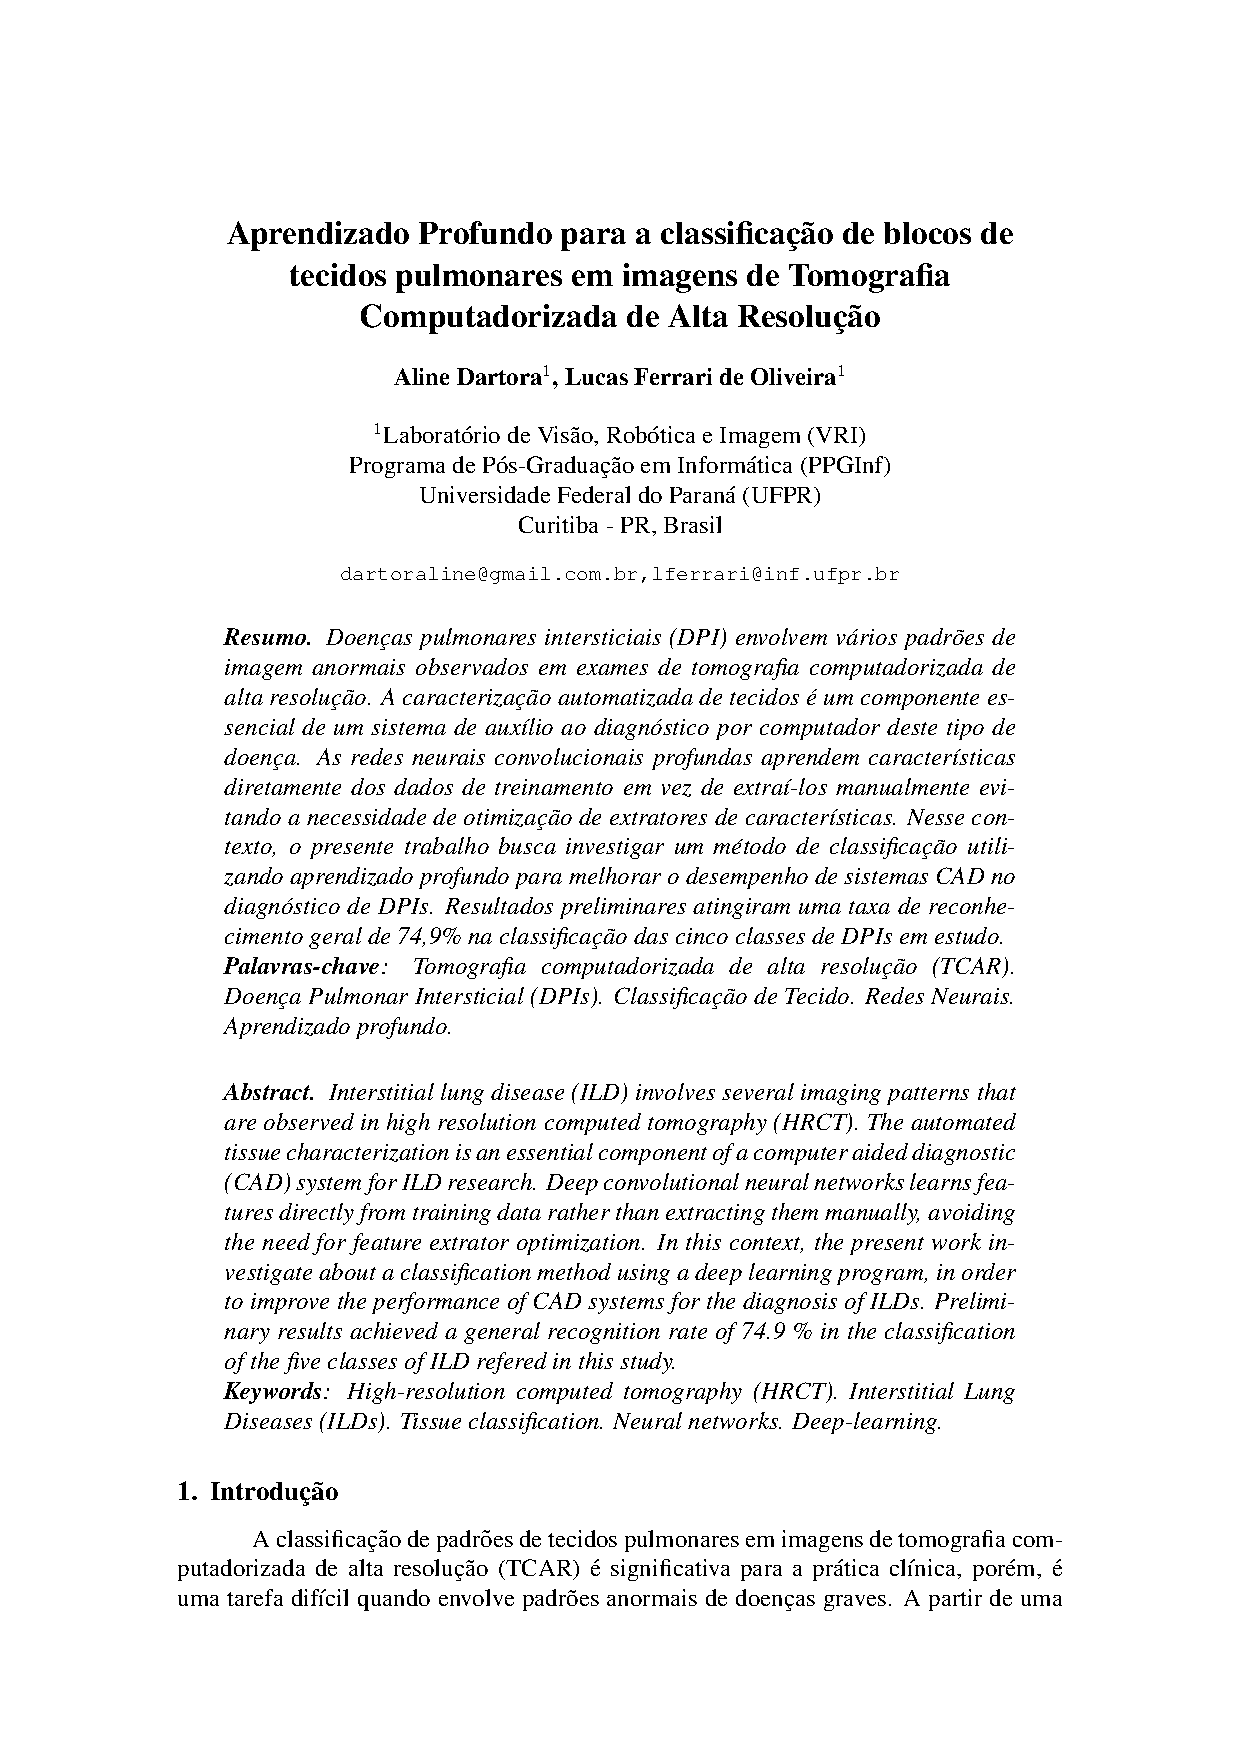
\includegraphics[width=0.3\textwidth]{./img/002}}
  \hspace{0.5cm}
  \subfloat[\ ]{\label{fig:exG53}\includegraphics[width=0.3\textwidth]{./img/003}}\\
  \small{Elaborado por Bacon}
\end{figure}





\section{Refer�ncias Bibliogr�ficas no Padr�o ABNT}

